\documentclass[journal,onecolumn]{IEEEtran}
\usepackage{url}
\usepackage{graphicx}
\usepackage{placeins}
\usepackage{float}
\usepackage{listings}
\usepackage{textcomp}
\usepackage{abstract}
\graphicspath{ {./img/} }


% *** GRAPHICS RELATED PACKAGES ***
%
\ifCLASSINFOpdf
  % \usepackage[pdftex]{graphicx}
  % declare the path(s) where your graphic files are
  % \graphicspath{{../pdf/}{../jpeg/}}
  % and their extensions so you won't have to specify these with
  % every instance of \includegraphics
  % \DeclareGraphicsExtensions{.pdf,.jpeg,.png}
\else
  % or other class option (dvipsone, dvipdf, if not using dvips). graphicx
  % will default to the driver specified in the system graphics.cfg if no
  % driver is specified.
  % \usepackage[dvips]{graphicx}
  % declare the path(s) where your graphic files are
  % \graphicspath{{../eps/}}
  % and their extensions so you won't have to specify these with
  % every instance of \includegraphics
  % \DeclareGraphicsExtensions{.eps}
\fi



% *** Do not adjust lengths that control margins, column widths, etc. ***
% *** Do not use packages that alter fonts (such as pslatex).         ***
% There should be no need to do such things with IEEEtran.cls V1.6 and later.
% (Unless specifically asked to do so by the journal or conference you plan
% to submit to, of course. )


% correct bad hyphenation here
\hyphenation{op-tical net-works semi-conduc-tor}


\begin{document}

% paper title
% can use linebreaks \\ within to get better formatting as desired
% Do not put math or special symbols in the title.

\title{Home Automation System Project Report }

\author{Vivek~Pujara,~\IEEEmembership{CS~807~Student,~University~of~Regina,}
\\~Mikhail~Shchukin,~\IEEEmembership{CS~807~Student,~University~of~Regina,}
\\~Gideon~Eromosele,~\IEEEmembership{CS~807~Student,~University~of~Regina,}
~and~Oluwatobi~Adegbola,~\IEEEmembership{CS~807~Student,~University~of~Regina,}
}


% The paper headers
% This should either be the name of the journal or the
% first four(ish) words of the paper
\markboth{CS 807 Project Report, April~17th~2019}%
{Shell \MakeLowercase{\textit{et al.}}: Design, Template, Computer Science }
% The only time the second header will appear is for the odd numbered pages
% after the title page when using the twoside option.


% make the title area
\maketitle

% As a general rule, do not put math, special symbols or citations
% in the abstract or keywords.
\begin{abstract}
This research project report provides a comprehensive overview on the concept of home automation, available hardware design for this topic, the motivation behind improving the base design, and the materials gathered for such improvement.
Consequently, the prototype design of the suggested home automation solution is discussed and demonstrated. Achieved project milestones and future work ideas are then explained.
\end{abstract}

% Note that keywords are not normally used for peerreview papers.
\begin{IEEEkeywords}
design, home automation, hardware, CS 807
\end{IEEEkeywords}



% For peer review papers, you can put extra information on the cover
% page as needed:
% \ifCLASSOPTIONpeerreview
% \begin{center} \bfseries EDICS Category: 3-BBND \end{center}
% \fi
%
% For peerreview papers, this IEEEtran command inserts a page break and
% creates the second title. It will be ignored for other modes.
\IEEEpeerreviewmaketitle



\section{Introduction}

\IEEEPARstart{H}{ome} automation today is a well-known concept introduced in 1998 and was majorly developed in the early 2000’s \textsuperscript{\cite{IEEEhowto:Hendricks}}. Since then many attempts have been made to design an automated control system that could be used in various buildings and environments.

Particularly, we use the base project from Arduino Project Hub named Home Automation Using Arduino and Bluetooth Control as a starting point \textsuperscript{\cite{IEEEhowto:Kumar}}. Basically, it is an Arduino-based system comprising of various sensors and actuators along with a Bluetooth module for remote control via mobile device. The features of the base project include remote conrol of lighting, doors, appliances and temperature regulation. Infrared and ultrasonic sensors are used for detecting human presence. Temperature sensor is used to monitor temperature inside the house. Servo motors and light emitting diodes are used to simulate the effects of controlling the automated parts of the house, represented by a miniature prototype.

The main motivation to attempt an improvement project in home automation system development is based on the increasing community interest in the Internet of Things (IoT) as a concept allowing to extend the automation of any system, including a typical residential building, to a considerably new level of integration.

The idea revolves around having a network of various actuators and sensors, in various settings, where the user has a remote control capability for basically any interactive component of such hardware network. Particularly, an automated home can be defined as a hardware-augmented dwelling, where various sensors are the inputs keeping track of the environment and user state and the automated parts (doors, lighting, security alarm, etc.) are the actuators, the outputs of the system, and these components are connected together via some processing unit, usually a microcontroller.

For example, such system gives the resident of such hardware-augmented dwelling an ability for a TV or some living room lights to turn on based on sensing the presence of the owner in the house. Home automation enables the owner with the extended control over the property, where some functions can be accessed remotely, and the system might be able to notify the owner of its state (intrusion alert, regular status notifications, troubleshooting and more). 

This research project strives to pick an existing hardware project related to the Internet of things and home automation and suggest meaningful modifications and improvements to the existing design.

\section{Background \& Base Project}

Our project is inspired by Shubham Kumar's home automation prototype built with Arduino microcontroller \textsuperscript{\cite{IEEEhowto:Kumar}}. His prototype features all of the basic functionalities expected from a typical home automation system. However, there is a large space for improvements to be made. The base project lacks security, has unnecessary redundancy in sensor usage (both infrared and ultrasonic sensors are used to detect motion) and lacks the integration of components in cases where some sensors could have served for more than just a single purpose/subsystem. 

Our design additions concentrated around improving the security of the system, light intensity control, automatic triggering of perimeter lights, temperature monitoring and controlling air conditioning systems, garage door control, and better system accessibility via Wi-Fi on smartphones. The mentioned base project inspired our team to attempt a home automation development project to reduce the inefficiencies, redundancies and omissions, and to offer a better quality solution, at least on a prototype level.  All these improvements are essential to sustain a comfortable, reliable and secure residential environment.

Home automation systems provide property owners the opportunity to monitor and control the state of their home with negligible latency \textsuperscript{\cite{IEEEhowto:Pavithra}}. Ideally, the introduction of home automation enhances various key features of a typical dwelling: security, power saving (especially for bigger appliances), accident prevention. Commercial products of home automation field are typically advertised with these features as key components of the highly technological dwellings of the future. Nevertheless, the real problem is that such products do not give the user any particular, in-depth idea of how the promoted home automation system operates while companies are advertising their products as complete solutions or particular subsystems. 

By using the open-source Arduino platform and widely available low-cost components combined with our design and implementation steps explained step by step in this report, our project also strives to increase awareness of the average user on the fundamental principles of home automation operation.

\section{Design process}

Throughout the development of this project, our team has encountered various design trade-offs, general issues and multiple decision factors that influenced our design. This section provides consequential explanation and analysis of our design process.

\subsection{System overview}

As we already mentioned, home automation is a rather complicated combination of sensors, actuators and the processing unit. In order to achieve proper functionality, desirable quality and consistent representation of the system, we resorted to modular, systematic design approach. As seen on Fig. \ref{fig:img2}, our home automation system is divided into several subsystems with different purposes.

\begin{figure}[H]
  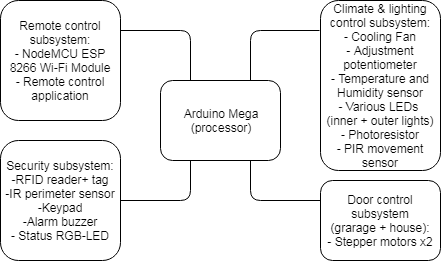
\includegraphics[width=0.5\textwidth]{img/img2.png}
  \caption{The logical structure of the project}
  \label{fig:img2}
\end{figure}

These four major subsystems are controlled via Arduino Mega microcontroller board. It is notable that smaller microcontroller boards of the same family (i.e. Arduino Uno) appeared to have insufficient amount of control pins for the designated modules to operate. 

After dividing the overall functionality of the desired home automation solution into related subsystems, it is easier to debug and develop these modules separately. 

\subsection{Materials Required}
The implementation of the suggested home automation system is a complex task that involves a wide variety of sensors, actuators and a multitude auxillary components. Below, we list the major electronic components that are required by the outlined design:
\begin{itemize}
	\item{Sensors:}
	\begin{itemize}
		\item{1x RC522 RFID reader and RFID-Tag}
		\item{1x Keypad}
		\item{1x Rotary Potentiometer}
		\item{4x Infrared sensors + emitters (square perimeter)}
		\item{1x Passive Infrared sensor w/lens dome}
		\item{1x Photoresistor}
		\item{1x RHT03 Temperature + Humidity Sensor Module}
		\item{1x Wi-Fi module (NodeMCU ESP8266)}
	\end{itemize}
	\item{Actuators:}
	\begin{itemize}
		\item{4x Green, 4x Orange LEDs}
		\item{1x RGB LED}
		\item{1x Alarm Buzzer}
		\item{1x LCD Screen}
		\item{2x 28BYJ-48 Stepper Motors}
		\item{2x X113647 Stepper Driver Boards}
		\item{1x DC Motor Fan}
	\end{itemize}
	\item{Miscellaneous:}
	\begin{itemize}
		\item{1x Arduino Mega 2560 (Microcontroller board)}
		\item{1x External power supply board}
		\item{1x big + 2x smaller Prototyping Breadboards}
		\item{Various Jumper Wires}
		\item{Various Resistors (1k$\Omega$)}
	\end{itemize}
\end{itemize}

\subsection{Security of the system}
Security is a major concern for every house owner. Thus, an ideal home automation system should have decent security in place. These security design elements contribute to the integrity and reliability of the system:
\begin{itemize}
    \item {Property access is only allowed after RFID-tag + Keypad code authentication process. A user provides a valid RFID-tag and then enters the code on the keypad. On incorrect password entry or 1 minute timeout, the system keeps scanning for the correct RFID-tag}
    \item {An alarm buzzer is in place. It is triggered when security system is on and the perimeter is breached. It can only be turned off with a button inside the house (it is assumed that such button is not in plain sight and is hard to identify/access by the intruder)}
    \item {The house perimeter is assumed to be square and is monitored by detection lines formed by IR emitter and receiver pairs}
    \item {Remote access application allows the user to toggle the perimiter detection for peaceful entry/leaving.}
\end{itemize}

Security of the controlled premises was one of the biggest improvements to the base project and also required a significant amount of design workload for successful implementation later on. Our GitHub repository also demonstrates that the considerable portion of microcontroller code is dedicated to RFID and keypad processing \cite{git:git}. 

\subsection{Design challenges}
During the design process, we have encountered several fundamental challenges that affected our final prototype later on. Here is a comprehensive list of the hardware limitations and other issues that influenced our design decisions:
\begin{itemize}
	\item{Our original design consideration revolved around displaying the output using LCD display. However, we had to replace it with a single RGB LED to just display the status of the RFID authentication. This is due to the fact that LCD controls act as a heavy load on the microprocessor, which, at times, resulted in system failures. A single RGB LED is much easier to control and it is still useful for interaction.}
	\item{The problem described above also revealed that without an LCD display, the humidity/temperature sensor values are hard to visualize using single LEDs. To compensate for this interactivity loss, the values of the sensor can still communicated with USB serial communication to the PC that also serves as a main power source for the system.}
	\item{Cooling fan together with stepper motors in action could easily drain the system's power and cause system failure, if launched simultaneously. A single auxillary power supply could not solve the problem, so removing the cooling fan from the design and powering the stepper motors from the auxillary power source worked out as best scenario.}
	\item{Rotary potentiometer is originally designed to control the temperature threshold past which the cooling fan has to be turned on. This part of the design was kept until the very end of development and implementation of the prototype. While it has no real use without a cooling fan in the proposed system, the potentiometer and the related code was kept as backup variant to control the system should a different configuration be considered.}
\end{itemize}

Given these challenges, some components of the original design had to be removed or disabled as reflected on Fig. \ref{fig:img1}. At the cost of these minor design simplifications, we achieved a guaranteed stability, reliability and security of the system. 

\section{Implementation}

In this section, we briefly outline the implementation process of the proposed design and the related information.

First and foremost, the proposed system heavily relies on NodeMCU ESP8266 Wi-Fi module, which enables the remote interactivity through smartphone application. Wi-Fi and Bluetooth are the two major means of medium range wireless communication, but Wi-Fi is chosen for communication as a considerably better protected communication protocol with less traffic congestion and generally longer range of operation. The chosen Wi-Fi module is capable to serve as an access point on its own or to be connected to a router and accessed through it, as seen of Fig. \ref{fig:img3}.

\begin{figure}[H]
  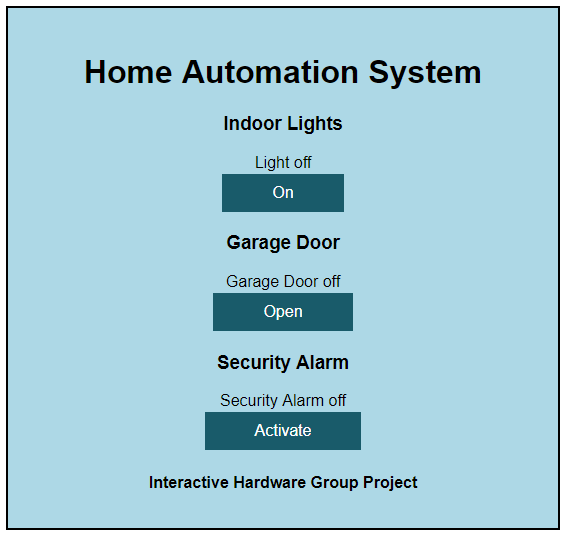
\includegraphics[width=0.5\textwidth]{img/img3.png}
  \caption{The interface of the remote control application (online)}
  \label{fig:img3}
\end{figure}

The app allows the user to have the following controls over the home automation system:
\begin{itemize}
	\item{Toggling the perimeter intrusion detection + alarm buzzer}
	\item{Opening/closing garage door}
	\item{Toggle indoor lights}
\end{itemize}

Depending on the received wireless command code, the microcontroller activates the requested chunk of code in a large switch statement, which gets executed immediately. When checking for the user input, the systems follows the general logic as outlined in Fig. \ref{fig:img4}

\begin{figure}[H]
  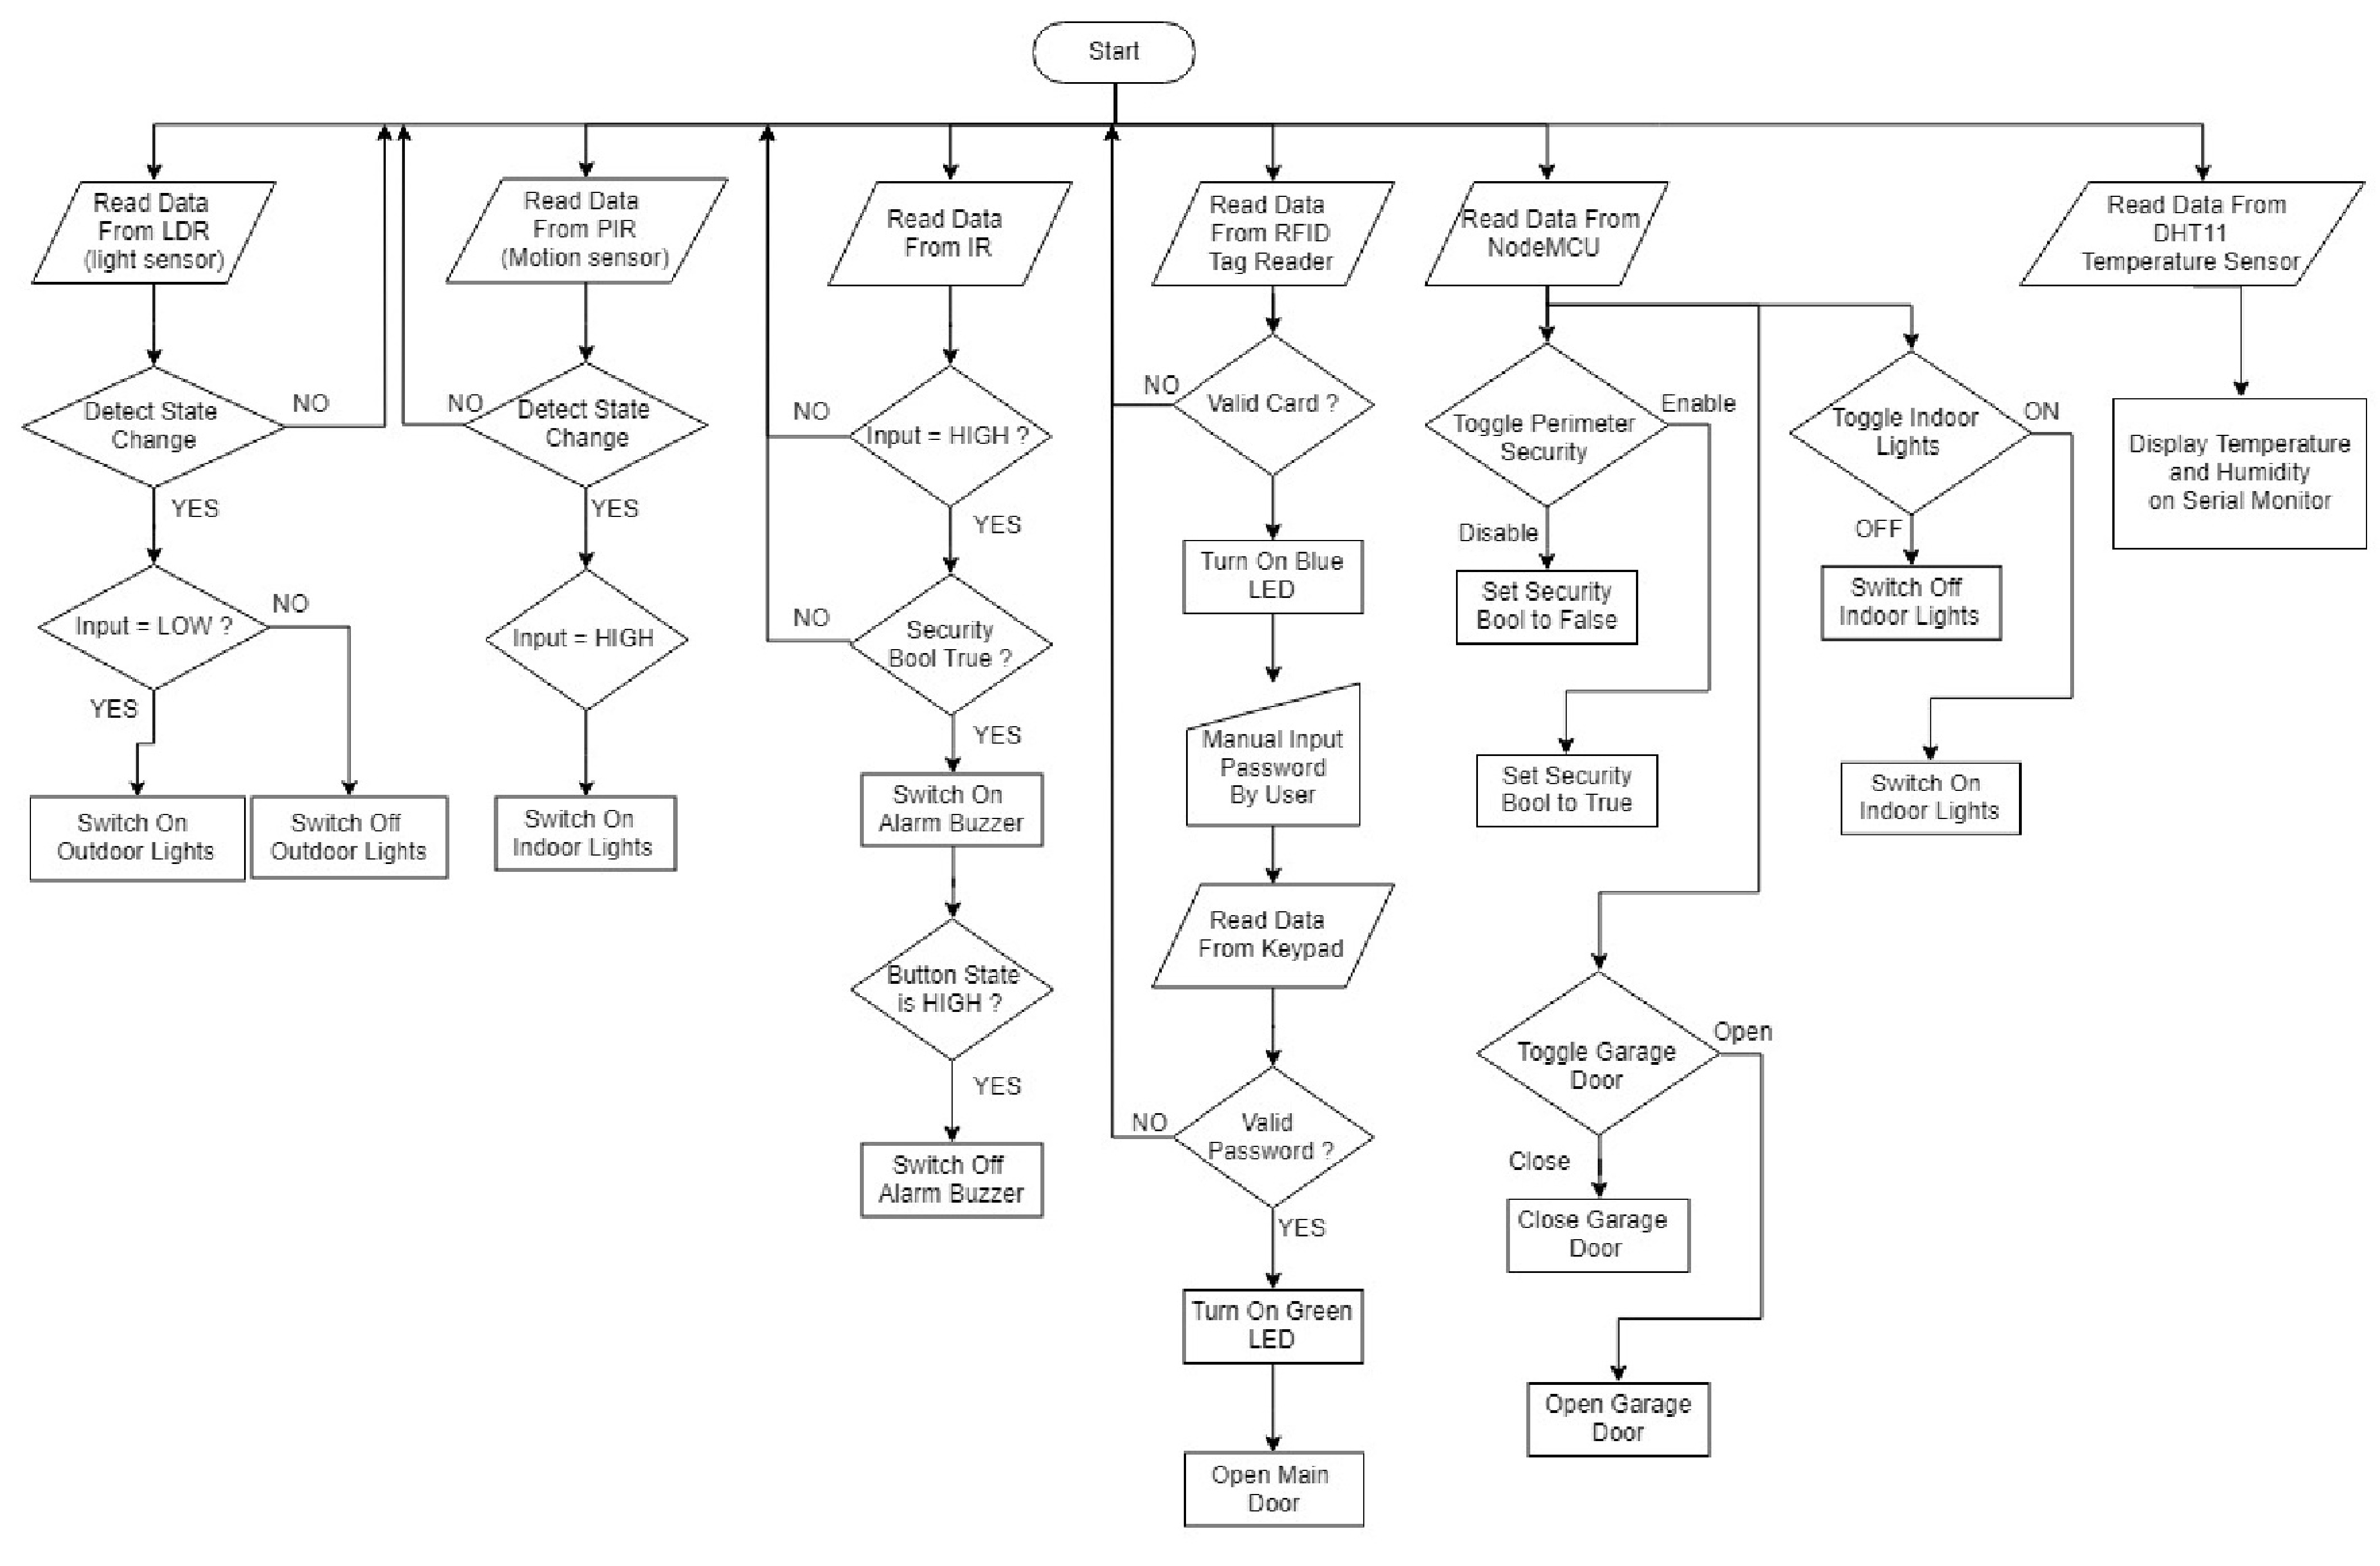
\includegraphics[width=0.8\textwidth]{img/img4.png}
  \caption{The general logic of the microcontroller code}
  \label{fig:img4}
\end{figure}

The final prototype was tested in scope of its designed functionality and fulfilled the expectations. Firstly, the user can deactivate perimeter security before entering the premises. Then, garage door stepper motor can open the garage when the user sends the signal from a vehicle outside the house. After that, when car is parked, the user may close the garage door and proceed to the house entrance with an RFID-tag. Once RFID-tag is accepted by the RFID-reader, the LED turns on, which indicates that the user may now enter the predefined password. Once a correct password is entered within a minute timeout, the door stepper motor automatically opens the door for the user. This concludes a typical use case of this home automation system when a user enters a house.

Similarly, if a user needs to leave the house, it is possible to send the remote control signal to open the garage door to access the car. When user is ready to go with the car outside the house, it is possible to close the garage door remotely and activate the perimeter security. Thus, we have achieved a full cycle of securing the premises with decent automation and remote control capabilities.

Aside from the described base functionality, the inner lights are controlled by a motion PIR sensor, so when entering the house, the user does not need to do extra work to physically access the lights switch. In case of perimeter breach alarm triggered and buzzer emitting loud noise, the user may access the hidden physical button inside the house to turn the alarm off after the breach is dealt with.

\section{Conclusion \& Future Work}

In the end of the development process, we have achieved a fully functional, presentable prototype. With all components mounted on a styrofoam miniature representation of a typical dwelling with garage, living room, smaller rooms and entrance doors. Remote control application launched on a smartphone can send the entirety of the designed commands. 

While we achieved a considerably better reliability, security and integrity of the system compared to the base project, there is still a considerable space for improvement. Particuarly, future projects on this topic should concentrate on powering issues to ensure that the components can work simultaneously without interfering with each other and threatening the system stability. Another important key improvement could be to add more functionality to the system together with scalablity. If there is a bigger number of appliances and other, more or less complicated actuators to contol, the system might need to rely on a distributed network of Arduino family microcontrollers that are linked into a bigger supersystem.

\subsection{Achievements}
The list below outlines the major milestones reached throughout the development of this project:
\begin{itemize}
	\item{\textbf{Milestone \#1:}}
		\begin{itemize}
		\item{Gathering the required materials}
		\item{\textbf{Result: Reached on time. No problems.}}
		\end{itemize}
	\item{\textbf{Milestone \#2:}}
		\begin{itemize}
		\item{Basic hardware assembly is done}
		\item{No meaningful code yet}
		\item{\textbf{Reached later than planned due to power issues.}}
		\end{itemize}
	\item{\textbf{Milestone \#3:}}
		\begin{itemize}
		\item{Sensors calibrated}
		\item{Various sensors/actuators are functional on their own}
		\item{Wireless networking is in active development}
		\item{\textbf{Result: Reached on time. Minor debugging issues.}}
		\end{itemize}
	\item{\textbf{Milestone \#4:}}
		\begin{itemize}
		\item{ A completely functional demo prototype is ready}
		\item{\textbf{Result: Reached later than planned due to design changes.}}
		\end{itemize}
	\item{\textbf{GOAL Milestone:}  }
		\begin{itemize}
		\item{Home Automated System final prototype works with all planned functionality and no failures}
		\item{The documentation of the implemented hardware design is finalized}
		\item{\textbf{Result: Reached on time. Minor debugging issues.}}
		\end{itemize}
\end{itemize}

As seen in this list, our team slightly underestimated the amount of workload that the debugging of various technical problems related to system power distribution, hardware assembly for the garage door opening mechanism and various software changes. Nevertheless, major milestones were met and the final, completely functional prototype has been delivered on time.

\subsection{Workload Distribution}
The project research, hardware design development and other tasks/roles are fulfilled by the research team as follows:
\begin{itemize}
\item{Vivek Pujara}
	\begin{itemize}
	\item{Lead Programmer}
	\item{Project Management Lead}
	\end{itemize}
\item{Mikhail Shchukin}
	\begin{itemize}
	\item{Documentation Lead Specialist}
	\item{Prototype Testing}
	\end{itemize}
\item{Gideon Eromosele}
	\begin{itemize}
	\item{Primary Hardware Designer}
	\item{Auxillary Programmer}
	\end{itemize}
\item{Oluwatobi Adegbola}
	\begin{itemize}
	\item{Auxillary Hardware Designer}
	\item{User Requirement Ellicitation}
	\end{itemize}
\end{itemize}

\subsection{Contributions}
Our team expresses sincere appreciation and gratitude to the following group of people that provided us with guidance, online materials, code examples and made considerable efforts to make this project happen:

\begin{itemize}
	\item{Trevor Tomesh -- in-person instruction, advising and inspiration}
	\item{Miguel Balboa -- RFID-related code samples and guidelines \cite{IEEEhowto:RFID}}
	\item{Rui Santos -- code for web server setup with NodeMCU and related instructions \cite{IEEEhowto:ESP}}
	\item{Rob Tillaart -- DHT library, code samples \cite{IEEEhowto:DHT}}
\end{itemize}

\appendices
\section{Diagrams and Pictures}

\begin{figure}[H]
  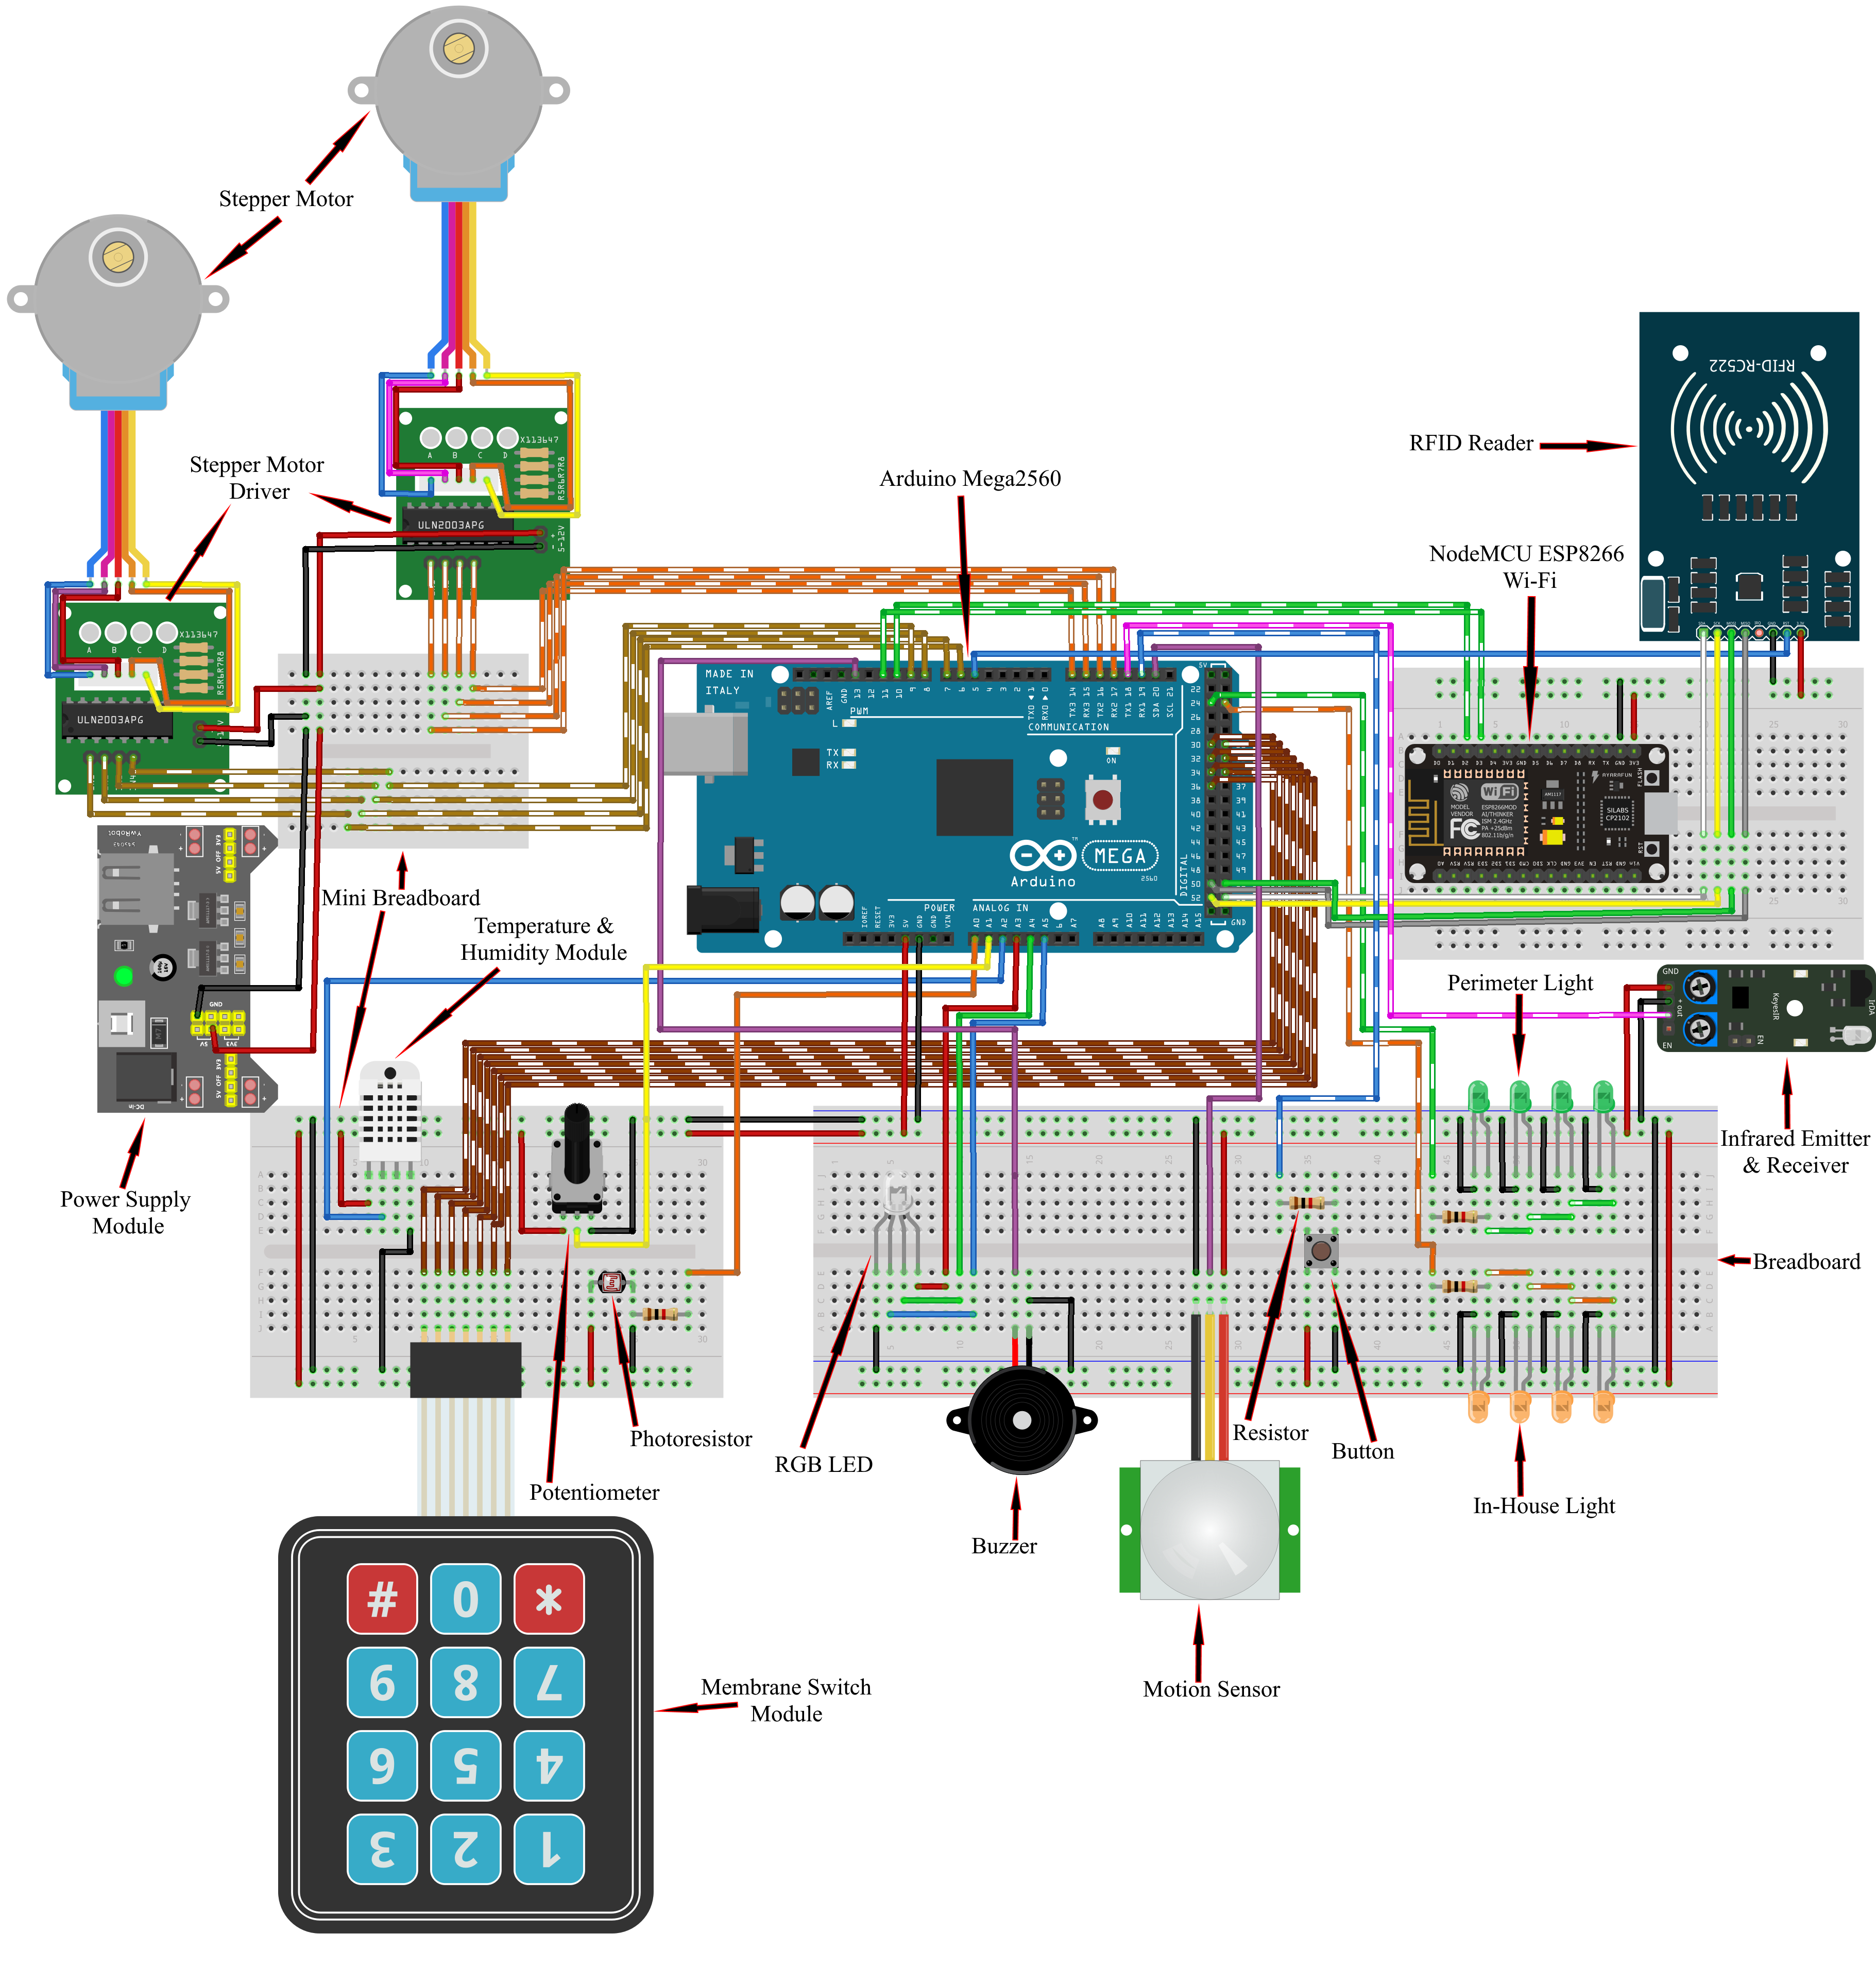
\includegraphics[width=\textwidth]{img/img1.png}
  \caption{The overall schematic of the project}
  \label{fig:img1}
\end{figure}

% you can choose not to have a title for an appendix
% if you want by leaving the argument blank


% THIS COULD HAVE BEEN A SEPARATE CODE APPENDIX,  
% BUT IT WAS REQUESTED THAT IT IS NOT DISPLAYED, SINCE GUTHUB REPO IS REFERENCED ALREADY
%\section{Source Code}
%\lstset{basicstyle=\ttfamily}
%\lstinputlisting[language=C++,breaklines=true]{code.ino}

% Can use something like this to put references on a page
% by themselves when using endfloat and the captionsoff option.
\ifCLASSOPTIONcaptionsoff
  \newpage
\fi

% references section

% can use a bibliography generated by BibTeX as a .bbl file
% BibTeX documentation can be easily obtained at:
% http://www.ctan.org/tex-archive/biblio/bibtex/contrib/doc/
% The IEEEtran BibTeX style support page is at:
% http://www.michaelshell.org/tex/ieeetran/bibtex/
%\bibliographystyle{IEEEtran}
% argument is your BibTeX string definitions and bibliography database(s)
%\bibliography{IEEEabrv,../bib/paper}
%
% <OR> manually copy in the resultant .bbl file
% set second argument of \begin to the number of references
% (used to reserve space for the reference number labels box)
\begin{flushleft}
\begin{thebibliography}{1}
\bibitem{git:git}
Eromsele, G., Pujara V. et al. (2019). \textit{Home Automation System} [online] GitHub. \\ Available at: \url{https://github.com/erogideon/Home-Automation-System} [Accessed 17 Apr. 2019].
\bibitem{IEEEhowto:Hendricks}
Hendricks, D. (2014). \textit{The History of Smart Homes.} [online] IoTEvolution. \\ Available at: \url{https://www.iotevolutionworld.com/m2m/articles/376816-history-smart-homes.htm} [Accessed 17 Apr. 2019].
\bibitem{IEEEhowto:Kumar}
Kumar, S. (2019). Home Automation Using Arduino and Bluetooth Control. [online] Arduino Project Hub. \\ Available at: \url{https://create.arduino.cc/projecthub/Shubhamkumar97/home-automation-using-arduino-and-bluetooth-control-404e9c?ref=user\&ref\_id=598721\&offset=0} [Accessed 17 Apr. 2019].
\bibitem{IEEEhowto:Pavithra}
Pavithra, D., Balakrishnan, R. (2015). \textit{IoT based monitoring and control system for home automation. Global Conference on Communication Technologies (GCCT)}. 169-173. doi: 10.1109/gcct.2015.7342646
\bibitem{IEEEhowto:RFID}
Balboa, M. (2019). \textit{Arduino RFID Library for MFRC522.} [online] GitHub. \\ Available at:  \url{https://github.com/miguelbalboa/rfid} [Accessed 17 Apr. 2019].
\bibitem{IEEEhowto:ESP}
Santos, R. (2019) \textit{Build an ESP8266 Web Server - Code and Schematics.} [online] Random Nerd Tutorials. \\ Available at: \url{randomnerdtutorials.com/esp8266-web-server/.} [Accessed 17 Apr. 2019].
\bibitem{IEEEhowto:DHT}
Tillaart, R. (2018). \textit{Class for DHTxx sensors (xx = 11-21-22-33-44).} [online] Arduino Playground. \\ Available at: \url{https://playground.arduino.cc/Main/DHTLib/} [Accessed 17 Apr. 2019].


\end{thebibliography}
\end{flushleft}

% that's all folks
\end{document}